\documentclass{book}
\usepackage{amsmath}
\usepackage{amssymb}
\usepackage{bm}
\usepackage{graphicx}
\usepackage{epstopdf}
\usepackage[bw]{mcode}
\usepackage{listings}
\DeclareGraphicsRule{.tif}{png}{.png}{`convert #1 `basename #1 .tif`.png}
\usepackage{color}
\pagestyle{plain}
%\pagestyle{empty}
\textheight 9 true in
\textwidth 6.5 true in
\hoffset -.75 true in
\voffset -.75 true in

\mathsurround=2pt  \parskip=2pt
\def\crv{\cr\noalign{\vskip7pt}}
\def\a{\alpha } \def\b{\beta } \def\d{\delta } \def\D{\Delta } \def\e{\epsilon }
\def\g{\gamma } \def\G{\Gamma} \def\k{\kappa} \def\l{\lambda } \def\L{\Lambda }
\def\th{\theta } \def\Th{\Theta} \def\r{\rho} \def\o{\omega} \def\O{\Omega}
\def\ve{\varepsilon}
\def\sech{\text{sech}}
\def\p{\partial}
\def\erf{\text{erf}}

\def\sA{{\cal A}} \def\sB{{\cal B}} \def\sC{{\cal C}} \def\sI{{\cal I}}
\def\sR{{\cal R}} \def\sF{{\cal F}} \def\sG{{\cal G}} \def\sM{{\cal M}}
\def\sT{{\cal T}} \def\sH{{\cal H}} \def\sD{{\cal D}} \def\sW{{\cal W}}
\def\sL{{\cal L}} \def\sP{{\cal P}} \def\s{\sigma } \def\S{\Sigma}
\def\sU{{\cal U}} \def\sV{{\cal V}} \def\sY{{\cal Y}}

\def\gm{\gamma -1}
\def\summ{\sum_{j=1}^4}

\def\bb{{\bm b}} \def\yb{{\bm y}}
\def\ub{{\bm u}}  \def\xb{{\bm x}} \def\vb{{\bm v}} \def\wb{{\bm w}}
\def\omegab{{\bm \omega}} \def\rb{{\bm r}} \def\ib{{\bm i}} \def\jb{{\bm j}}
\def\lb{{\bm l}} \def\kb{{\bm k}} \def\Ab{{\bm A}} \def\fb{{\bm f}} \def\Ub{{\bm U}}
\def\Fb{{\bm F}} \def\nb{{\bm n}} \def\Db{{\bm D}} \def\eb{{\bm e}}
\def\gb{{\bm g}}  \def\Gb{{\bm G}} \def\hb{{\bm h}} \def\Yb{{\bm Y}} \def\Rb{{\bm R}}
\def\Tb{{\bm T}}

\def\As1{{\bf {\cal A}}_1}\def\DO{{\cal D}_0} \def\UO{{\cal U}_0}
\def\ie{{\it{i.e.}}}

\def\ubbar{{\bf {\bar{u}}}} \def\sbar{{\bar{\sigma }}} \def\ubar{{\bar{u}}}
\def\abar{{\bar{a}}} \def\vbar{{\bar{v}}}  \def\rbar{{\bar{\rho}}}
\def\pbar{{\bar{p}}} \def\ebar{{\bar{e}}} \def\Tbar{{\bar{T}}}
\def\bbar{{\bar{\beta}}} \def\Mbar{{\bar{M}}}  \def \sMbar{{\bar{\cal M}}}
\def\Ebar{{\bar{E}}} \def\sMbar{{\bar{\cal M}}}
\def\sPbar{{\bar{\cal P}}} \def\xbar{{\bar{x}}}

\newcommand{\pdv}[2]{\frac{\partial#1}{\partial#2}}
\newcommand{\dv}[2]{\frac{d#1}{d#2}}
\newcommand{\ord}[2]{#1^{(#2)}}
\newcommand{\vct}[1]{\vec{#1}}

 \newcommand{\bc}{\begin{center}}
 \newcommand{\ec}{\end{center}}

 \newcommand{\bq}{\begin{equation}}
 \newcommand{\eq}{\end{equation}}

 \newcommand{\beqs}{\begin{eqnarray}}
 \newcommand{\eeqs}{\end{eqnarray}}

 \newcommand{\beqa}{\begin{eqnarray*}}
 \newcommand{\eeqa}{\end{eqnarray*}}

 \newcommand{\ol}{\overline}
 \newcommand{\ul}{\underline}

 \newcommand{\dint}{{\int \!\! \int \!\!}}
 \newcommand{\tint}{{\int \!\! \int \!\! \int \!\!}}

 \newcommand{\bfig}{\begin{figure}}
 \newcommand{\efig}{\end{figure}}

 \newcommand{\cen}{\centering}
 \newcommand{\n}{\noindent}

 \newcommand{\btab}{\begin{table}}
 \newcommand{\etab}{\end{table}}

 \newcommand{\btbl}{\begin{tabular}}
 \newcommand{\etbl}{\end{tabular}}

 \newcommand{\bdes}{\begin{description}}
 \newcommand{\edes}{\end{description}}

 \newcommand{\benum}{\begin{enumerate}}
 \newcommand{\eenum}{\end{enumerate}}

 \newcommand{\bite}{\begin{itemize}}
 \newcommand{\eite}{\end{itemize}}

 \newcommand{\cle}{\clearpage}
 \newcommand{\npg}{\newpage}

 \newcommand{\bss}{\begin{singlespace}}
 \newcommand{\ess}{\end{singlespace}}

 \newcommand{\bhalf}{\begin{onehalfspace}}
 \newcommand{\ehalf}{\end{onehalfspace}}

 \newcommand{\bds}{\begin{doublespace}}
 \newcommand{\eds}{\end{doublespace}}

 \newcommand{\eps}{\mbox{$\epsilon$}}
 \newcommand{\stilde}{\mbox{$\tilde s$}}
 \newcommand{\shat}{\mbox{$\hat s$}}

 \newcommand{\blue}{\color{blue}}
 \newcommand{\red}{\color{red}}
 \newcommand{\magenta}{\color{magenta}}
 \newcommand{\green}{\color{green}}
 \newcommand{\nc}{\normalcolor}




\pagestyle{empty}
\begin{document}

\begin{center}
\large{ MATH-6890 \hspace{1in} Numerical Solutions of Waves  \hspace{1in}Fall 2016 \\ Due Thursday September 22, 2016.}\end{center}
Michael Hennessey

\bigskip
\bc {\bf Problem Set 3} \ec
\benum 
	\item Consider the initial value problem
	$$u_{tt}=c^2(u_{xx}+u_{yy})$$
	subject to appropriate initial conditions. Note here that $c$ is assumed real.
	\benum
		\item Determine the dispersion relation and general form of the exact solutions.\\
		
		Solution:\\
		
		We make the ansatz $u=\exp(i(k_x x+k_y y-\o t))$ to find the equation
		\bq (-i\o)^2=c^2[(ik_x)^2+(ik_y)^2]\eq
		which simplifies to the dispersion relations
		\bq \o=\pm c\sqrt{k_x^2+k_y^2}.\eq
		Then $u$ takes the form
		\bq u=A\exp[i(k_x x+k_y y-c\sqrt{k_x^2+k_y^2}t)]+B\exp[i(k_x x+k_y 				  y+c\sqrt{k_x^2+k_y^2}t)].\eq
		
		\item We use a centered, second-order accurate discretization in both space and time to determine the numerical dispersion relation. We then determine the time-step restriction of the method.\\
		
			Solution:\\
			
			We let $u(x_j,y_k,t_n)=u_{j,k}^n$ be our discrete variables.
			Since no spatial domain has been specified, we assume an infinite domain. 
			Thus we can apply the discrete Fourier transform to find the dispersion relation.
			We begin by finding the explicit discrete equation in time:
			$$D_+^tD_-^t u_{j,k}^n=c^2(D_+^xD_-^xu_{j,k}^n+D_+^yD_-^yu_{j,k}^n)$$
			which simplifies to 
			\bq u_{j,k}^{n+1}=2u_{j,k}^n-u_{j,k}^n+\frac{c^2\Delta t^2}{\Delta x^2}
				[u_{j+1,k}^n-2u_{j,k}^n+u_{j-1,k}^n]+\frac{c^2\Delta^2}{\Delta y^2}
				[u_{j,k+1}^n-2u_{j,k}^n+u_{j,k-1}^n].\eq
			We define
			$$\s=\frac{c\Delta t}{\Delta x}\;\;\text{ and }\;\; \l=\frac{c\Delta t}{\Delta y}$$
			for simplification. Then we can use the discrete Fourier transform in both space variables:
			$$\hat{u}^n(\xi,\eta)=\frac{1}{2\pi}\sum_{j=-\infty}^\infty\sum_{k=-\infty}^\infty 
				\exp[-i(j\xi+k\eta)]u_{j,k}^n.$$
			This results in the transformations:
			$$u_{j,k}^{n+1}\to \hat{u}^{n+1},\;\; u_{j,k}^{n-1}\to \hat{u}^{n-1},$$
			$$u_{j+1,k}^n\to e^{i\xi}\hat{u}^n,\;\; u_{j-1,k}^n=e^{-i\xi}\hat{u}^n,$$
			$$u_{j,k+1}^n\to e^{i\eta}\hat{u}^n,\;\; u_{j,k-1}^n=e^{-i\eta}\hat{u}^n.$$
			Substituting the transformed variables into the equation (4) results in the equation
			\bq \hat{u}^{n+1}=2\hat{u}^n-\hat{u}^{n-1}+\s^2\hat{u}^n\left[e^{i\xi}-2+
				e^{-i\xi}\right]+\l^2\hat{u}^n\left[e^{i\eta}-2+e^{-i\eta}\right].\eq
			After some simplification, we can find a quadractic-like equation:
			$$\hat{u}^{n+1}-2\hat{u}^n[\s^2(\cos\xi-1)+\l(\cos\eta-1)+1]+\hat{u}^{n-1}=0.$$
			We then assume solutions of the form $\hat{u}^n=\r^n(\xi,\eta)\hat{u}^0(\xi,\eta).$ 
			This results in the quadratic equation for $\rho$:
			\bq \rho^2-2\rho[1-\s^2(1-\cos\xi)-\l^2(1-\cos\eta)]+1=0.\eq
			We then let $b=1-\s^2(1-\cos\xi)-\l^2(1-\cos\eta)$, and we see that $\rho$ 
			has solutions of the form
			\bq \rho=\frac{2b\pm\sqrt{4b^2-4}}{2}=b\pm\sqrt{b^2-1}\eq
			which is the numerical dispersion relation for the difference equation. 
			For this relation to result in stable solutions, we require $b^2-1<0.$ 
			We then expand $b^2$ to see
			$$\s^4(1-\cos\xi)^2+2\s^2\l^2(1-\cos\xi)(1-\cos\eta)
				-2\s^2(1-\cos\xi)-2\l^2(1-\cos\eta)+\l^4(\cos\eta-1)^2<0.$$
			If we then look at the case where $\eta=\xi$ we get significant simplification to the point where we get to
			$$2(\s^2+\l^2)>(\s^2+\l^2)^2(1-\cos\xi).$$
			We then argue that since $\max(1-\cos\xi)=2$ we have
			$$2(\s^2+\l^2)\geq2(\s^2+\l^2)^2$$
			hence we have
			$$1\geq \s^2+\l^2.$$
			Simplifiying this expression results in the time-step bound:
			\bq \Delta t\leq \frac{\Delta x\Delta y}{|c|\sqrt{\Delta x^2+\Delta y^2}}.\eq
			
			
			\item Create surface plots of the symbol vs. wave numbers for fixed time step. Select a variety of representative $\s$ and $\l$ that give both stable and unstable schemes. Discuss your results paying particular attention to which Fourier modes are the first to become unstable.\\
			
			Solution:\\
			
			The surface plots are included at the beginning of the next page.
			\begin{figure}
			\centering
			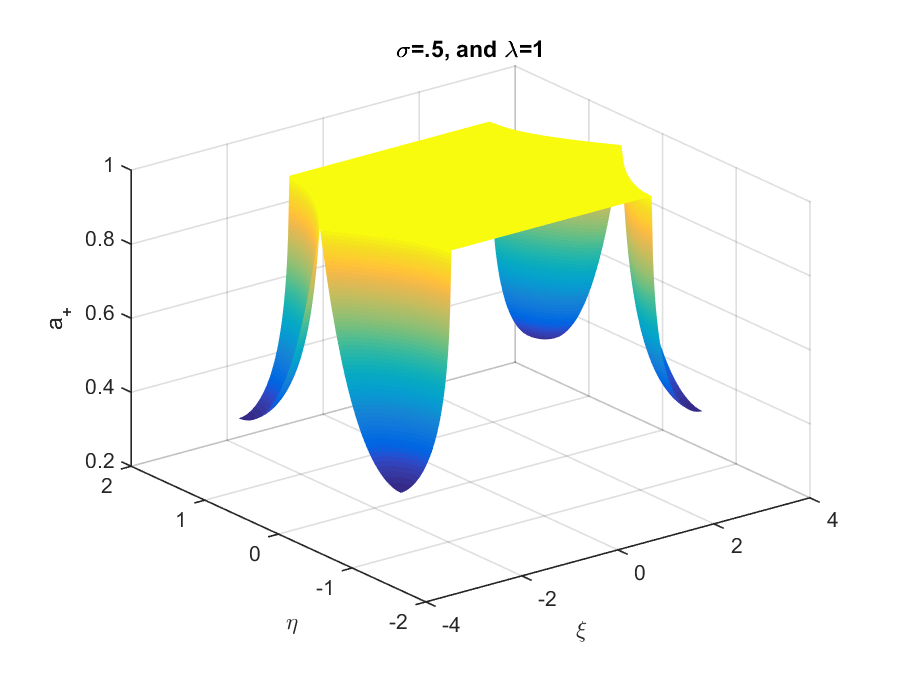
\includegraphics[width=3in]{symvwav1p}
			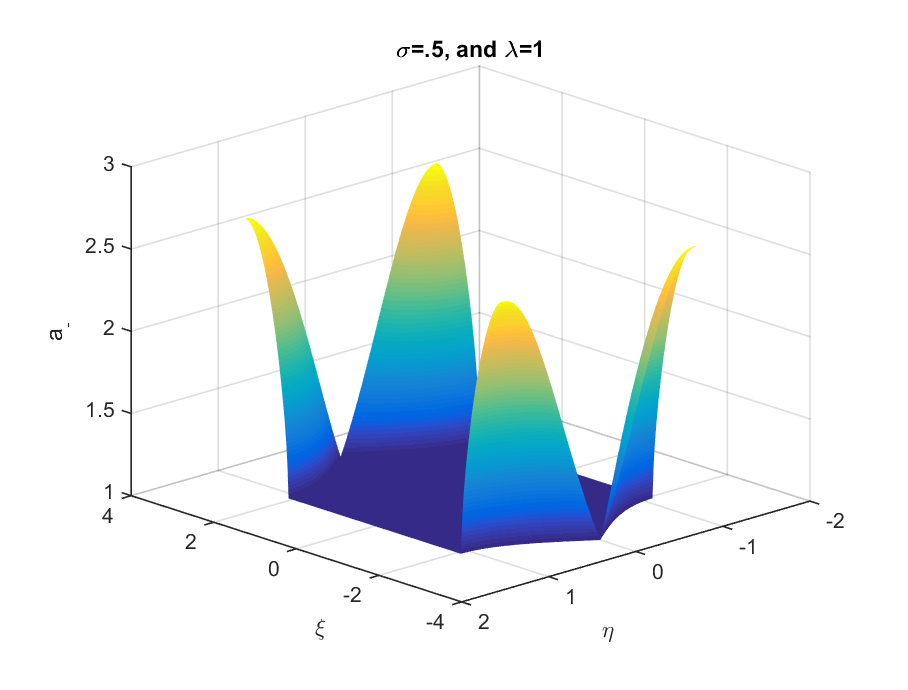
\includegraphics[width=3in]{symvwav1m}\\
			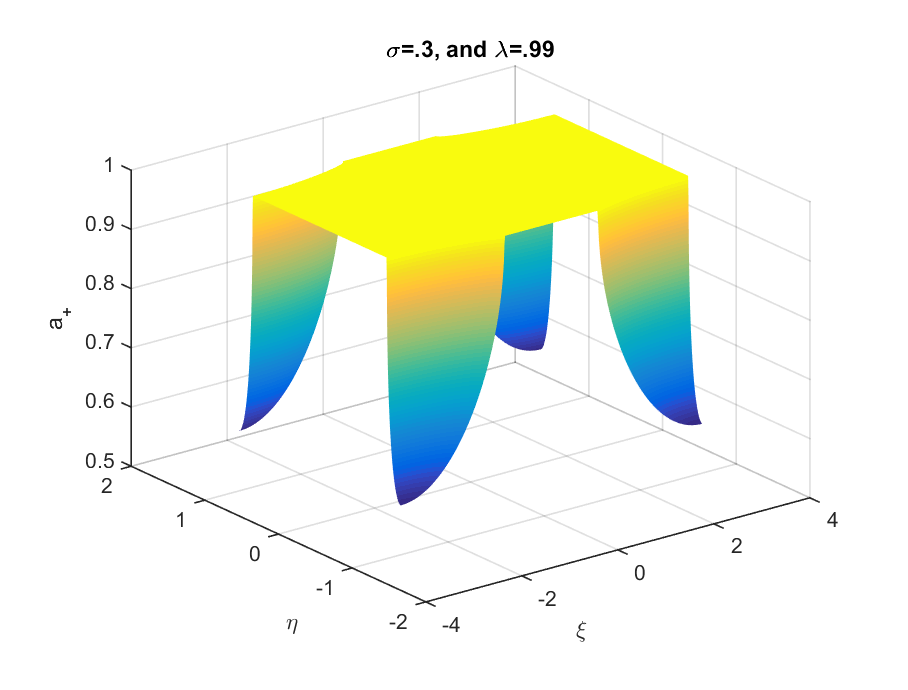
\includegraphics[width=3in]{symvwav2p}
			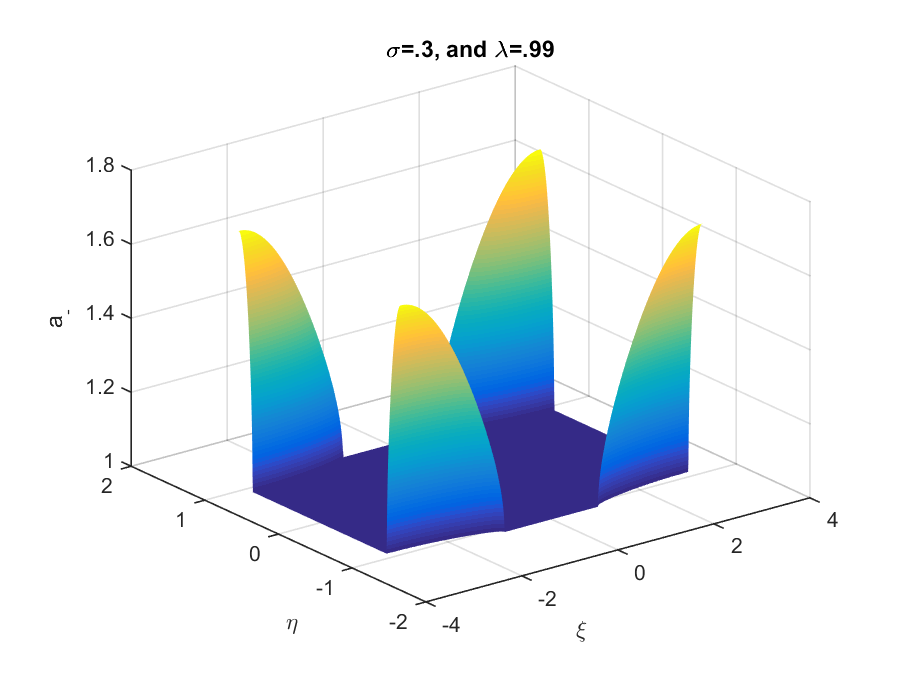
\includegraphics[width=3in]{symvwav2m}\\
			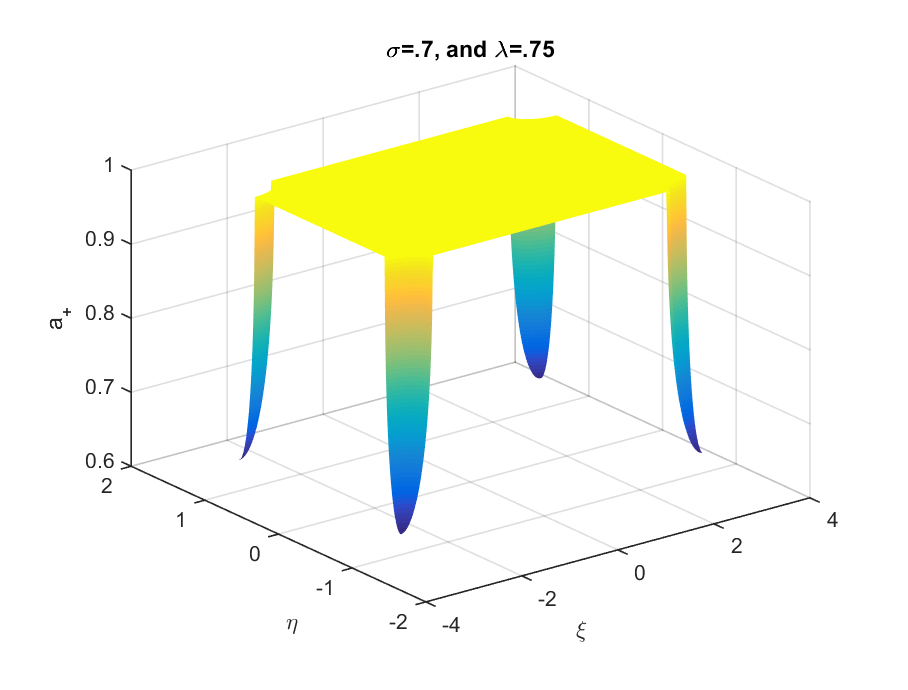
\includegraphics[width=3in]{symvwav3p}
			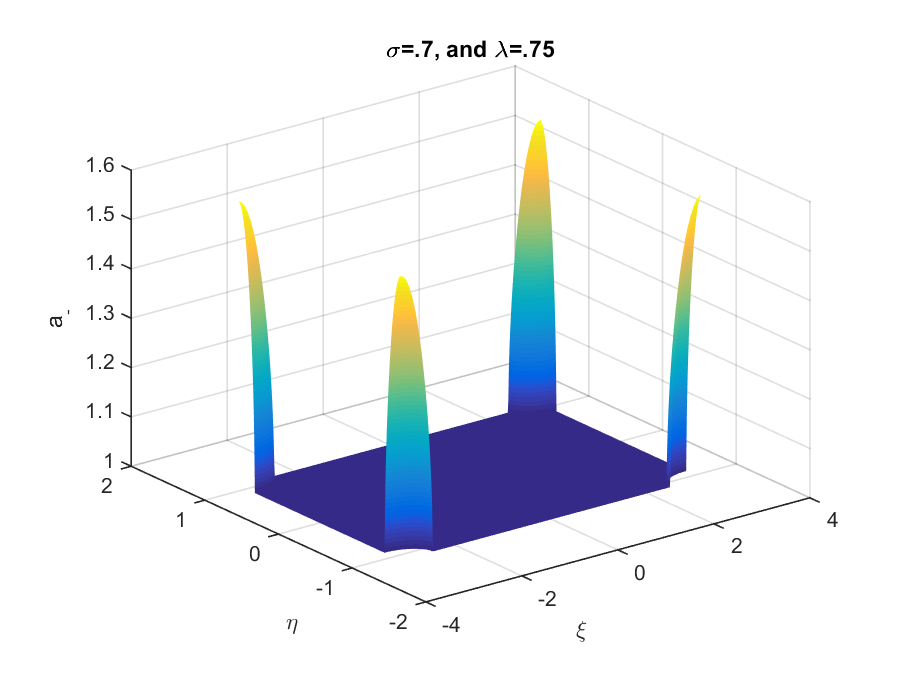
\includegraphics[width=3in]{symvwav3m}
			\end{figure}
			
			We can see then that the Fourier modes which become unstable depend largely upon the values of $\l$ and $\s$. If, for example, $\l\approx 1$ and $\s<<1$, we see almost uniform stability in $\xi$ modes, but only a very narrow range of stable modes in $\eta.$ The converse is obviously true. However, if $\l\approx\s$, we see a wide range of stable modes for each. In fact, for any $\l,\s<.7$, we see uniform stability for any $\xi,$ $\eta$ pair in $[-\pi,\pi]$. 
			\eenum
			\pagebreak
		\item Consider the initial-boundary value problem
		$$u_{tt}=c^2(u_{xx}+u_{yy}),\;\;\; 0<x<\pi,\;\;\;0<y<\pi,\;\;\;t>0$$
		with initial and boundary conditions
		\begin{align*}
		u(0,y,t)=u(\pi,y,t)=0\\
		u_y(x,0,t)=u_y(x,\pi,t)=0\\
		u(x,y,0)=2\sin(x)\cos(y)\\
		u_t(x,y,0)=-\sqrt{2}c\cos(x)\cos(y)+\sqrt{2}c\cos(x)\cos(y).
		\end{align*}
		Note this corresponds to the exact standing wave solution
		$$u=\sin(x-\sqrt{2}ct)\cos(y)+\sin(x+\sqrt{2}ct)\cos(y)$$
		which is the superposition of a left-going and right-going wave.\\
		In MATLAB, develop a centered, second-order accurate code to solve this problem. Boundary conditions should be treated via compatibility, and the time-step selected based on your results from (1b) above. Using the maximum norm, perform a grid convergence study with $c=1$ and $t_f=1$ to demonstrate second-order accuracy. In addition, plot both the approximate solution and numerical errors at $t=0.1,t=1, $ and $t=2.$\\
		
		Solution:\\
		
		The code and its desired results are presented here, along with the run code, the convergence study code, and the resulting loglog plot.\\
		
		MATLAB centered, second-order accurate code:
		\begin{lstlisting}
		function [err,dx,dy]=waveD2(M,N,xa,xb,ya,yb,c,tf,iPlot)

%% Set Global variables
global dx dy dt ng ja jb ka kb x y Mtot Ntot

%% Initialize grid
dx=(xb-xa)/M;
dy=(yb-ya)/N;
dt=.9*(dx*dy)/(c*sqrt(dx^2+dy^2));
Nt=ceil(tf/dt);
dt=tf/Nt;
%assign ghost points
ng=1;

% data set for grid
Mtot=M+1+2*ng;
ja=ng+1;
jb=Mtot-ng;

Ntot=N+1+2*ng;
ka=ng+1;
kb=Ntot-ng;

x=linspace(xa-ng*dx,xb+ng*dx,Mtot);
y=linspace(ya-ng*dx,yb+ng*dx,Ntot);

%% set Initial conditions
[unm1,un]=setICs;

%% allocate space for u

u=zeros(size(un));
if iPlot==1
    figure
end



%% Loop through time
t=dt;
for n=1:Nt-1
    
    %% Set boundary conditions on current step
    un=setBCs(un,t);
    %% Compute update over domain interior
    for j=ja:jb
        for k=ka:kb
            %uxx=-(sin(x(j)-sqrt(2)*c*t)*cos(y(k))+sin(x(j)+sqrt(2)*c*t)*cos(y(k)));
            %uyy=-uxx;
            uxx=(un(j+1,k)-2*un(j,k)+un(j-1,k))/dx^2;
            uyy=(un(j,k+1)-2*un(j,k)+un(j,k-1))/dy^2;
            utt=uxx+uyy;
            u(j,k)=2*un(j,k)-unm1(j,k)+c^2*dt^2*utt;
            %u(j,k)=(sin(x(j)-sqrt(2)*c*t)*cos(y(k))+sin(x(j)+sqrt(2)*c*t)*cos(y(k)));
        end
    end

    %% Update solution histories
    unm1=un;
    un=u;
    t=t+dt;
    %% Plot stuff
    if iPlot==1
        plotStuff(u,t)
    end
    
    
    %% Calculate exact solution and check error
    ue=uex(t);
    xind=ja:jb;
    yind=ka:kb;
    
    err=max(max(abs(u(xind,yind)-ue(xind,yind))));
    %err=norm(u(xind,yind)-ue(xind,yind),1);
    

end




%% Define boundary functions and derivatives
    function z=gl(~,~)
        z=0;
    end
    function z=gr(~,~)
        z=0;
    end
    function z=gltt(~,~)
        z=0;
    end
    function z=grtt(~,~)
        z=0;
    end
    function z=bl(~,~)
        z=0;
    end
    function z=br(~,~)
        z=0;
    end
    function z=f(m,n)
        z=2*sin(m)*cos(n);
    end
    function z=g(a,b)
        z=-sqrt(2)*c*cos(a)*cos(b)+sqrt(2)*c*cos(a)*cos(b);
    end
    function z=fxx(a,b)
        z=-2*sin(a)*cos(b);
    end
    function z=fyy(a,b)
        z=-2*sin(a)*cos(b);
    end

    function z=uex(t)
        z=zeros(M,N);
        for a=ja:jb
            for b=ka:kb
                z(a,b)=sin(x(a)-sqrt(2)*c*t)*cos(y(b))+sin(x(a)+sqrt(2)*c*t)*cos(y(b));
            end
        end
    end
%% Initial condition function
    function [unm1,un]=setICs
        
        %Set intitial condition at t=0:
        unm1=zeros(Mtot,Ntot);
        for a=ja:jb
            for b=ka:kb
                unm1(a,b)=f(x(a),y(b));
            end
        end
        
        unm1=setBCs(unm1,0);
        
        
        %% Initialize at t=dt
        %% we use a Taylor expansion in time
        un=zeros(Mtot,Ntot);
        for a=ja:jb
            for b=ka:kb
                un(a,b)=f(x(a),y(b))+dt*g(x(a),y(b))+...
                    c^2*dt^2/2*(fxx(x(a),y(b))+fyy(x(a),y(b)));
                %un(a,b)=sin(x(a)-sqrt(2)*c*dt)*cos(y(b))+sin(x(a)+sqrt(2)*c*dt)*cos(y(b));
            end
        end
        un=setBCs(un,dt);
        return
    end
%% Boundary condition function
    function un=setBCs(un,t)
        for a=ka:kb
            uyyl=(un(ja,a+1)-2*un(ja,a)+un(ja,a-1))/dy^2;
            %uyyl=-(sin(x(ja)-sqrt(2)*c*t)*cos(y(a))+sin(x(ja)+sqrt(2)*c*t)*cos(y(a)));
            un(ja-1,a)=2*un(ja,a)-un(ja+1,a)+dx^2/c^2*gltt(y(a),t)-dx^2*uyyl;
            
            uyyr=(un(jb,a+1)-2*un(jb,a)+un(jb,a-1))/dy^2;
            %uyyr=-(sin(x(jb)-sqrt(2)*c*t)*cos(y(a))+sin(x(jb)+sqrt(2)*c*t)*cos(y(a)));
            un(jb+1,a)=2*un(jb,a)-un(jb-1,a)+dx^2/c^2*grtt(y(a),t)-dx^2*uyyr;
        end
        for b=ja:jb
            un(b,ka-1)=un(b,ka+1)-2*dy*bl(x(b),t);
            un(b,kb+1)=un(b,kb-1)+2*dy*br(x(b),t);
        end
    end

%% Plot function
    function plotStuff(u,t)
        ue=uex(t);
        xind=ja:jb;
        yind=ka:kb;
        subplot(2,1,1)
        surf(x(xind),y(yind),u(xind,yind))
        hold on
        surf(x(xind),y(yind),ue(xind,yind))
        xlabel('x');
        ylabel('y');
        zlabel('u');
        hold off
        
        subplot(2,1,2)
        surf(u(xind,yind)-ue(xind,yind))
        xlabel('x')
        ylabel('y')
        zlabel('error');
        drawnow;
        pause
        return
    end
end
\end{lstlisting}

MATLAB run code:
\begin{lstlisting}
  N = 40;
  M = 40;
  xa = 0;
  xb = pi;
  ya = 0;
  yb = pi;
  c = 1;
  tf = 1;
  iPlot=0;
  [err,dx,dy]=waveD2(M,N,xa,xb,ya,yb,c,tf,iPlot);
\end{lstlisting}
\vspace{.4in}
Convergence study code:
\begin{lstlisting}
N0 = 20;

xa = 0;
xb = pi;
ya=0;
yb=pi;
c = 1;
tf = 1;
m = 4;

hPlot   = zeros(m,1);
errPlot = zeros(m,1);
kPlot=zeros(m,1);

for k = 0:m-1
    N = N0*2^k;
    M=N;
   [errPlot(k+1),hPlot(k+1),kPlot(k+1)]=waveD2(M,N,xa,xb,ya,yb,c,tf,0);

end

loglog( hPlot,errPlot,'x', hPlot,(hPlot.^3), 'g-');
figure
loglog(kPlot,errPlot,'x',kPlot,(kPlot.^2)/35,'k-');
\end{lstlisting}

Convergence Study results are found here. We see the code is slightly better than 2nd order accurate from this study, but it is not 3rd order accurate
\begin{figure}[ht]
\centering
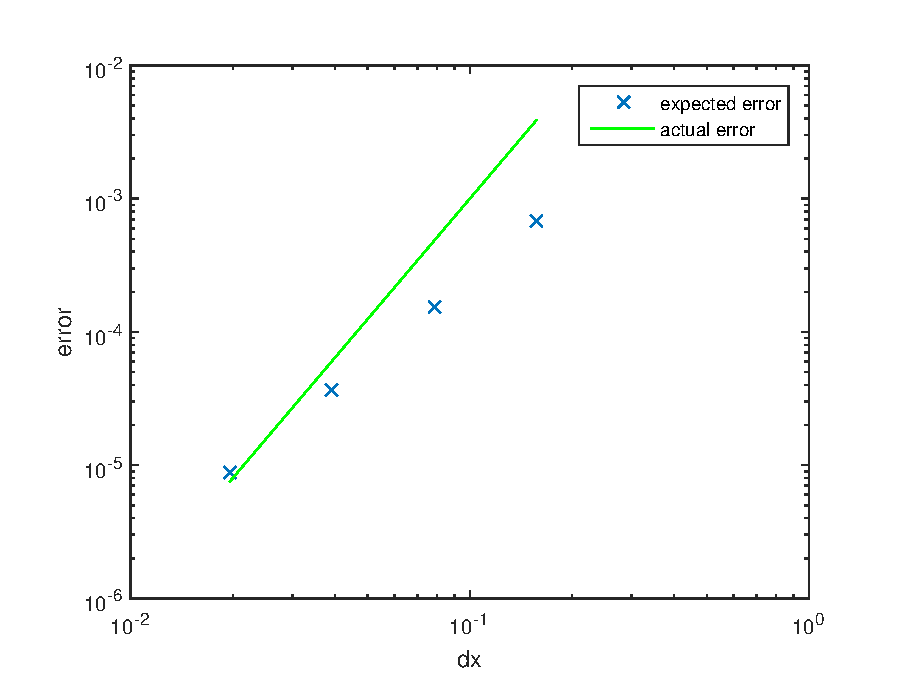
\includegraphics[width=3in]{convstdx}
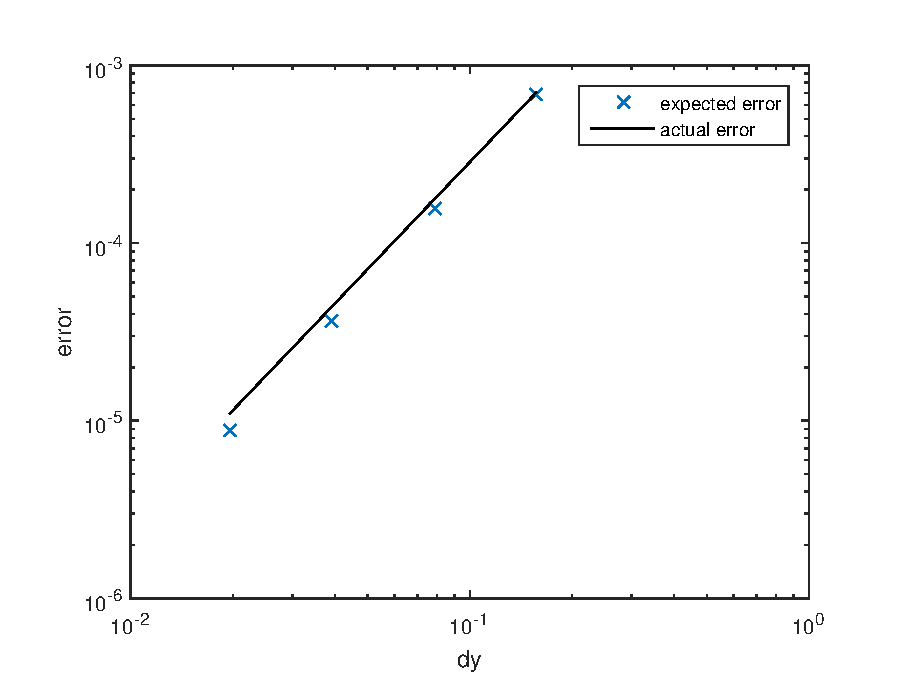
\includegraphics[width=3in]{convstdy}
\end{figure}

The solutions at $t=.1,1,2$ are found on the next page.
\begin{figure}
\centering
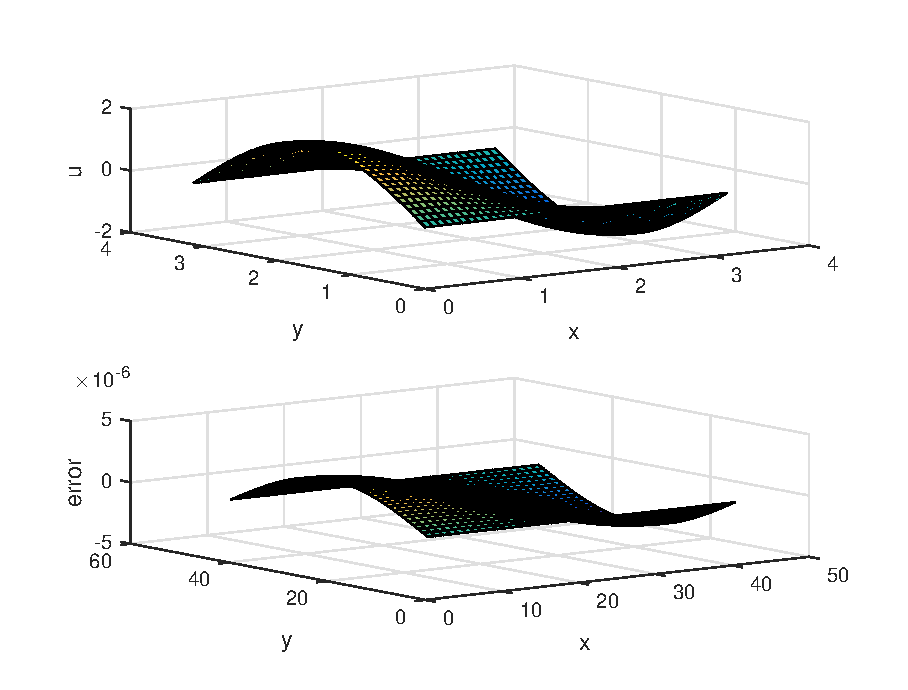
\includegraphics[width=4in]{solnt01}
\caption{Solutions and Error at $t=0.1$}
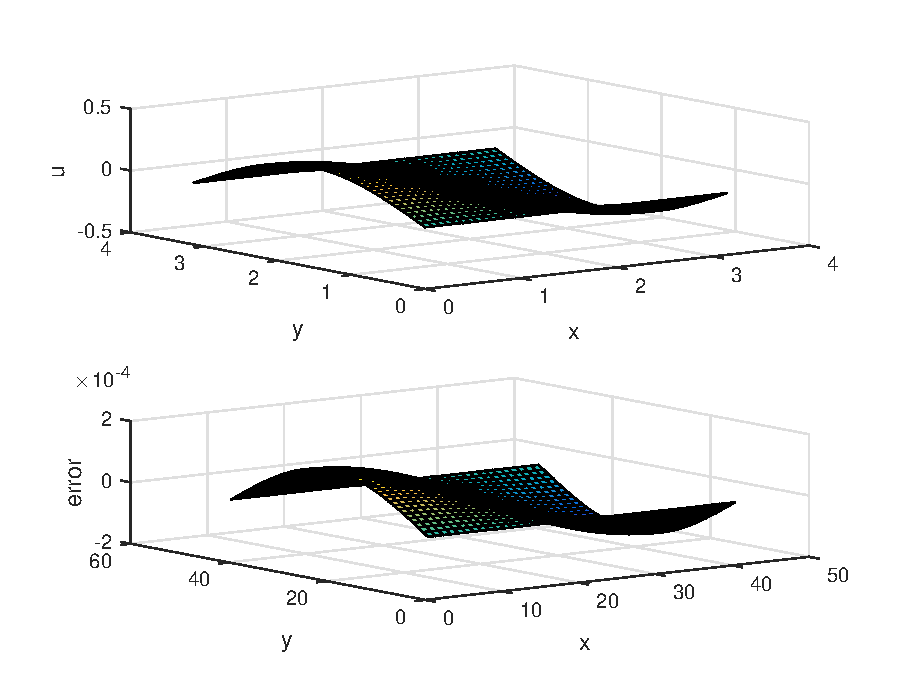
\includegraphics[width=4in]{solnt1}\\
\caption{Solutions and Error at $t=1$}
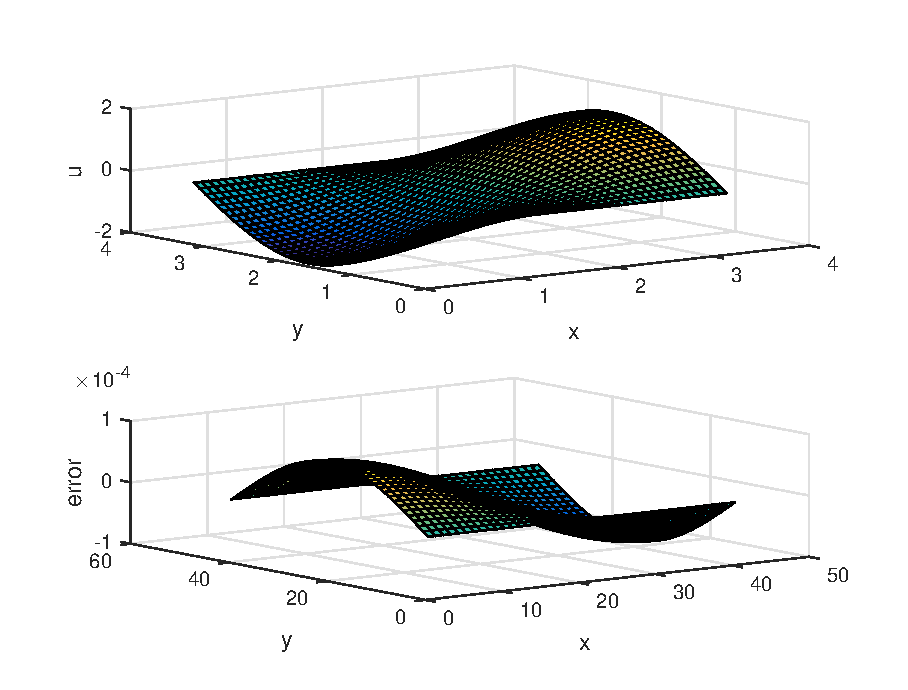
\includegraphics[width=4in]{sonlt2}
\caption{Solutions and Error at $t=2$}
\end{figure}

		\pagebreak
		\item Repeat exercise (2) with a C code.\\
		
		Solution:\\
		
		The C code is presented here:
		\begin{lstlisting}[language=C]
		/* Calculates Numerical Solution to the 2D wave equation */

#include<stdio.h>
#include<math.h>
#include<stdlib.h>
#include<time.h>

double main(void)
{
	double xa=0;
	double xb=3.1415926535897;
	double ya=0;
	double yb=3.1415926535897;
	double c=1;
	double tf=1;
	int M=160;
	int N=160;
	int ng=1;
	int Mtot=M+1+2*ng;
	int Ntot=N+1+2*ng;
	double dx=(xb-xa)/M;
	double dy=(yb-ya)/N;
	double dt;
	int ja;
	int jb;
	int ka;
	int kb;
	double x[Mtot];
	double y[Ntot];
	double unm1[Mtot][Ntot];
	double un[Mtot][Ntot];
	double u[Mtot][Ntot];
	double ue[M][N];
	double Nt;
	int i;
	int a;
	int b;
	int j;
	int k;
	double xj;
	double yk;
	double uyyr;
	double uyyl;
	double uxx;
	double uyy;
	double utt;
	double maxerr;
	double err;
	double stperr;
	double t=0;
	
	dt=.9*(dx*(double)dy)/(c*sqrt(dx*(double)dx+dy*(double)dy));
	//printf("%lf\n",dt);
	Nt=ceil(tf/(double)dt);
	//printf("%lf\n",Nt);
	
	dt=tf/(double)Nt;
	//printf("%lf",dt);
	
	ja=ng;
	jb=Mtot-ng-1;
	ka=ng;
	kb=Ntot-ng-1;
	//printf("%d, %d, %d, %d\n",ja,jb,ka,kb);
	
	/* Define grid*/
	
	for(i=0;i<Mtot;i++)
	{
		x[i]=dx*(double)(i-1);
	}
	
	for (i=0;i<Ntot;i++)
	{
		y[i]=dy*(double)(i-1);
	}
	//printf("%lf \n", x[41]);
	
	/* Set Initial Conditions and check error*/
	//maxerr=0;
	for(a=ja;a<=jb;a++)
	{
		xj=x[a];
		for(b=ka;b<=kb;b++)
		{	
			yk=y[b];
			unm1[a][b]=2*(double)sin(xj)*(double)cos(yk);
			//ue[a][b]=cos(yk)*(double)(sin(xj-sqrt(2)*(double)c*(double)t)+sin(xj)-sqrt(2)*(double)c*(double)t);
			//stperr=fabs(ue[a][b]-unm1[a][b]);
			//if(stperr>maxerr)
			//{
			//	maxerr=stperr;
			//}
		}
	}
	//printf("Initial error is: %lf\n",maxerr);
	
	/*for(b=ka;b<=kb;b++)
	{
		printf("%lf %d\n",unm1[jb][b],b);
	}/*
	
	/* Set BCs for u(x,y,0)*/
	for(a=ka;a<=kb;a++)
	{
		uyyl=(unm1[ja][a+1]-2*(double)unm1[ja][a]+unm1[ja][a-1])/(double)dy/(double)dy;
		unm1[ja-1][a]=2*(double)unm1[ja][a]-unm1[ja+1][a]-dx*(double)dx*(double)uyyl;
		uyyr=(unm1[jb][a+1]-2*(double)unm1[jb][a]+unm1[jb][a-1])/(double)dy/(double)dy;
		unm1[jb+1][a]=2*(double)unm1[jb][a]-unm1[jb-1][a]-dx*(double)dx*(double)uyyr;
		//printf("%lf, %d\n",unm1[jb+1][a],a);
	}
	for(b=ja;b<=jb;b++)
	{
		unm1[b][ka-1]=unm1[b][ka+1];
		unm1[b][kb+1]=unm1[b][kb-1];
		//printf("%lf, %lf, %d\n,",unm1[b][ka-1], unm1[b][kb+1],b);
	}

	/* Check error once BCs installed
	maxerr=0;
	for(a=ja+1;a<=jb-1;a++)
	{
		for(b=ka+1;b<=kb-1;b++)
		{
			stperr=fabs(unm1[a][b]-ue[a][b]);
			if(stperr>maxerr)
			{
				maxerr=stperr;
			}
		}
	}
	printf("Initial error is %lf\n",maxerr);
	
	/* Initialize at t=dt*/
	for(a=ja;a<=jb;a++)
	{
		xj=x[a];
		for(b=ka;b<=kb;b++)
		{
			yk=y[b];
			un[a][b]=2*(double)sin(xj)*(double)cos(yk)
				-c*(double)c*(double)dt*(double)dt*
				(double)(4*(double)sin(xj)*(double)cos(yk))/(double)2;
			//printf("%lf %d,%d\n",un[a][b],a,b);	
		}
	}

	/* Set BCs for u(x,y,dt)*/
	for(a=ka;a<=kb;a++)
	{
		uyyl=(un[ja][a+1]-2*(double)un[ja][a]+un[ja][a-1])/(double)dy/(double)dy;
		un[ja-1][a]=2*(double)un[ja][a]-un[ja+1][a]-dx*(double)dx*(double)uyyl;
		uyyr=(un[jb][a+1]-2*(double)un[jb][a]+un[jb][a-1])/(double)dy/(double)dy;
		un[jb+1][a]=2*(double)un[jb][a]-un[jb-1][a]-dx*(double)dx*(double)uyyr;
		//printf("%lf, %lf , %d\n",un[ja-1][a],un[jb+1][a],a);
	}
	for(b=ja;b<=jb;b++)
	{
		un[b][ka-1]=un[b][ka+1];
		un[b][kb+1]=un[b][kb-1];
		//printf("%lf, %lf %d\n",un[b][ka-1],un[b][kb+1],b);
	}
	
	
	/*Loop Through Time*/
	t=dt;
	while(t<tf-.1*dt)
	{
		/*Set Boundary conditions on current step*/
		
		for(a=ka;a<=kb;a++)
		{
			uyyl=(un[ja][a+1]-2*(double)un[ja][a]+un[ja][a-1])/(double)dy/(double)dy;
			un[ja-1][a]=2*(double)un[ja][a]-un[ja+1][a]-dx*(double)dx*(double)uyyl;
			uyyr=(un[jb][a+1]-2*(double)un[jb][a]+un[jb][a-1])/(double)dy/(double)dy;
			un[jb+1][a]=2*(double)un[jb][a]-un[jb-1][a]-dx*(double)dx*(double)uyyr;
			//printf("%lf, %lf , %d\n",un[ja-1][a],un[jb+1][a],a);
		}
		for(b=ja;b<=jb;b++)
		{
			un[b][ka-1]=un[b][ka+1];
			un[b][kb+1]=un[b][kb-1];
			//printf("%lf, %lf %d\n",un[b][ka-1],un[b][kb+1],b);
		}
		
		/* Compute Update over Domain Interior*/
		for(j=ja;j<=jb;j++)
		{
			for (k=ka;k<kb+1;k++)
			{
				uxx=(un[j+1][k]-2*(double)un[j][k]+un[j-1][k])/(double)dx/(double)dx;
				uyy=(un[j][k+1]-2*(double)un[j][k]+un[j][k-1])/(double)dy/(double)dy;
				utt=uxx+uyy;
				u[j][k]=2*(double)un[j][k]-unm1[j][k]+c*(double)c*(double)dt*(double)dt*(double)utt;
			}
		}
		
		/* Update Solution Histories*/
		t=t+dt;
		for(j=ja;j<=jb;j++)
		{
			for(k=ka;k<=kb;k++)
			{
				unm1[j][k]=un[j][k];
				un[j][k]=u[j][k];
			}
		}
		
		
		/* Calculate exact solution and check error*/
		for(a=ja;a<=jb;a++)
		{
			xj=x[a];
			for(b=ka;b<=kb;b++)
			{
				yk=y[b];
				ue[a][b]=sin(xj-sqrt(2)*(double)c*(double)t)*(double)cos(yk)
						+sin(xj+sqrt(2)*(double)c*(double)t)*(double)cos(yk);
						
			}
		}
		maxerr=0;
		FILE *f = fopen("wave.txt","w");
		for(a=ja+1;a<=jb-1;a++)
		{
			for(b=ka+1;b<=kb-1;b++)
			{
				stperr=fabs(ue[a][b]-un[a][b]);
				fprintf(f, "%d %d %lf %lf %lf\n",a,b,u[a][b],ue[a][b],stperr);
				if(stperr>maxerr)
					maxerr=stperr;
			}
		}
		fclose(f);
		printf("The error at time %lf is %lf with dx=%lf\n",t,maxerr,dx);
		
	}	
	return 0;
}
\end{lstlisting}
The code was compiled using gcc. The solutions at the desired times are included on the next page. They were plotted using the MATLAB script presented below:
\begin{lstlisting}
fid=fopen('wave.txt','r');
A=fscanf(fid,'%f',[5,inf])';
for i=1:39
    for j=1:39
        U(i,j)=A(39*(i-1)+j,3);
        UE(i,j)=A(39*(i-1)+j,4);
        ERR(i,j)=A(39*(i-1)+j,5);
    end
end
x=linspace(0,pi,39);
y=linspace(0,pi,39);
subplot(2,1,1)
surf(x,y,U)
hold on
surf(x,y,UE)
xlabel('x');
ylabel('y');
zlabel('u');
hold off
subplot(2,1,2)
surf(x,y,ERR)
xlabel('x');
ylabel('y');
zlabel('error');
\end{lstlisting}

The convergence study plot is presented here. The convergence study was done using the same grid refinement as in the previous section. However, we can see that the C code is actually 3rd order accurate.
\begin{figure}[ht]
\centering
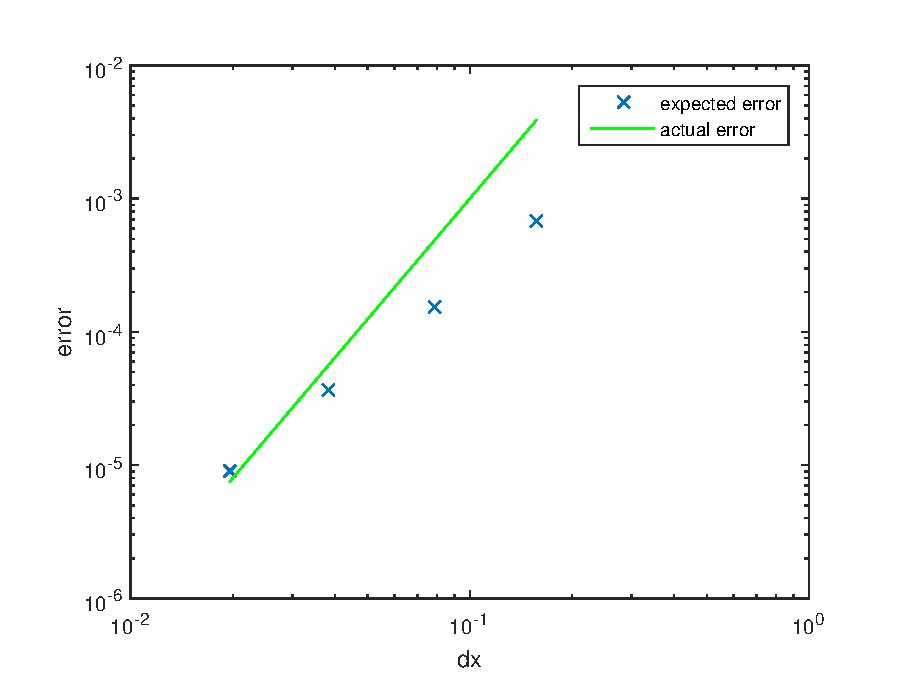
\includegraphics[width=3in]{cconvstdx}
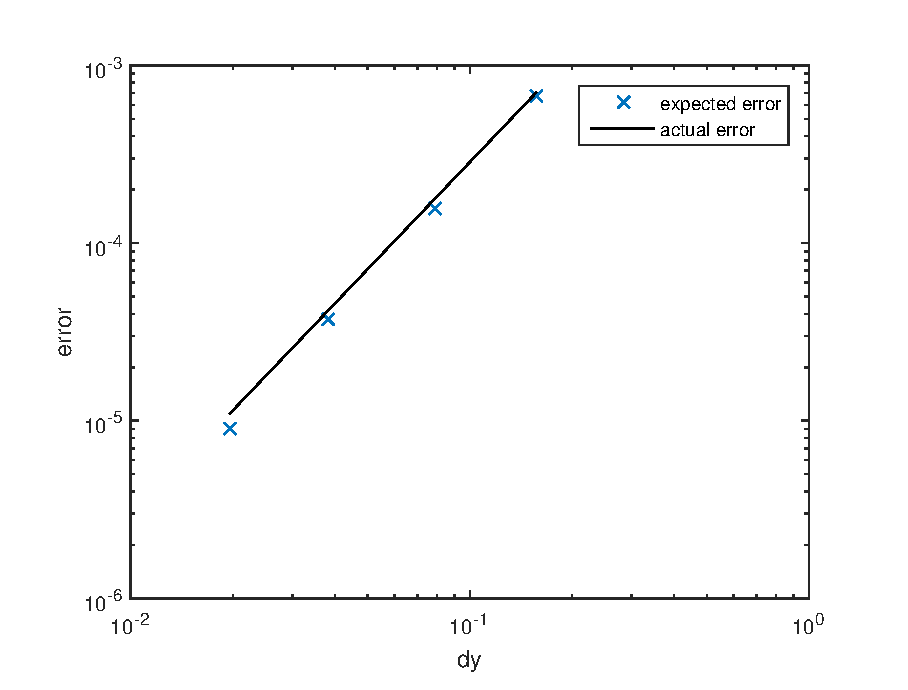
\includegraphics[width=3in]{cconvstdy}
\end{figure}
\begin{figure}
\centering
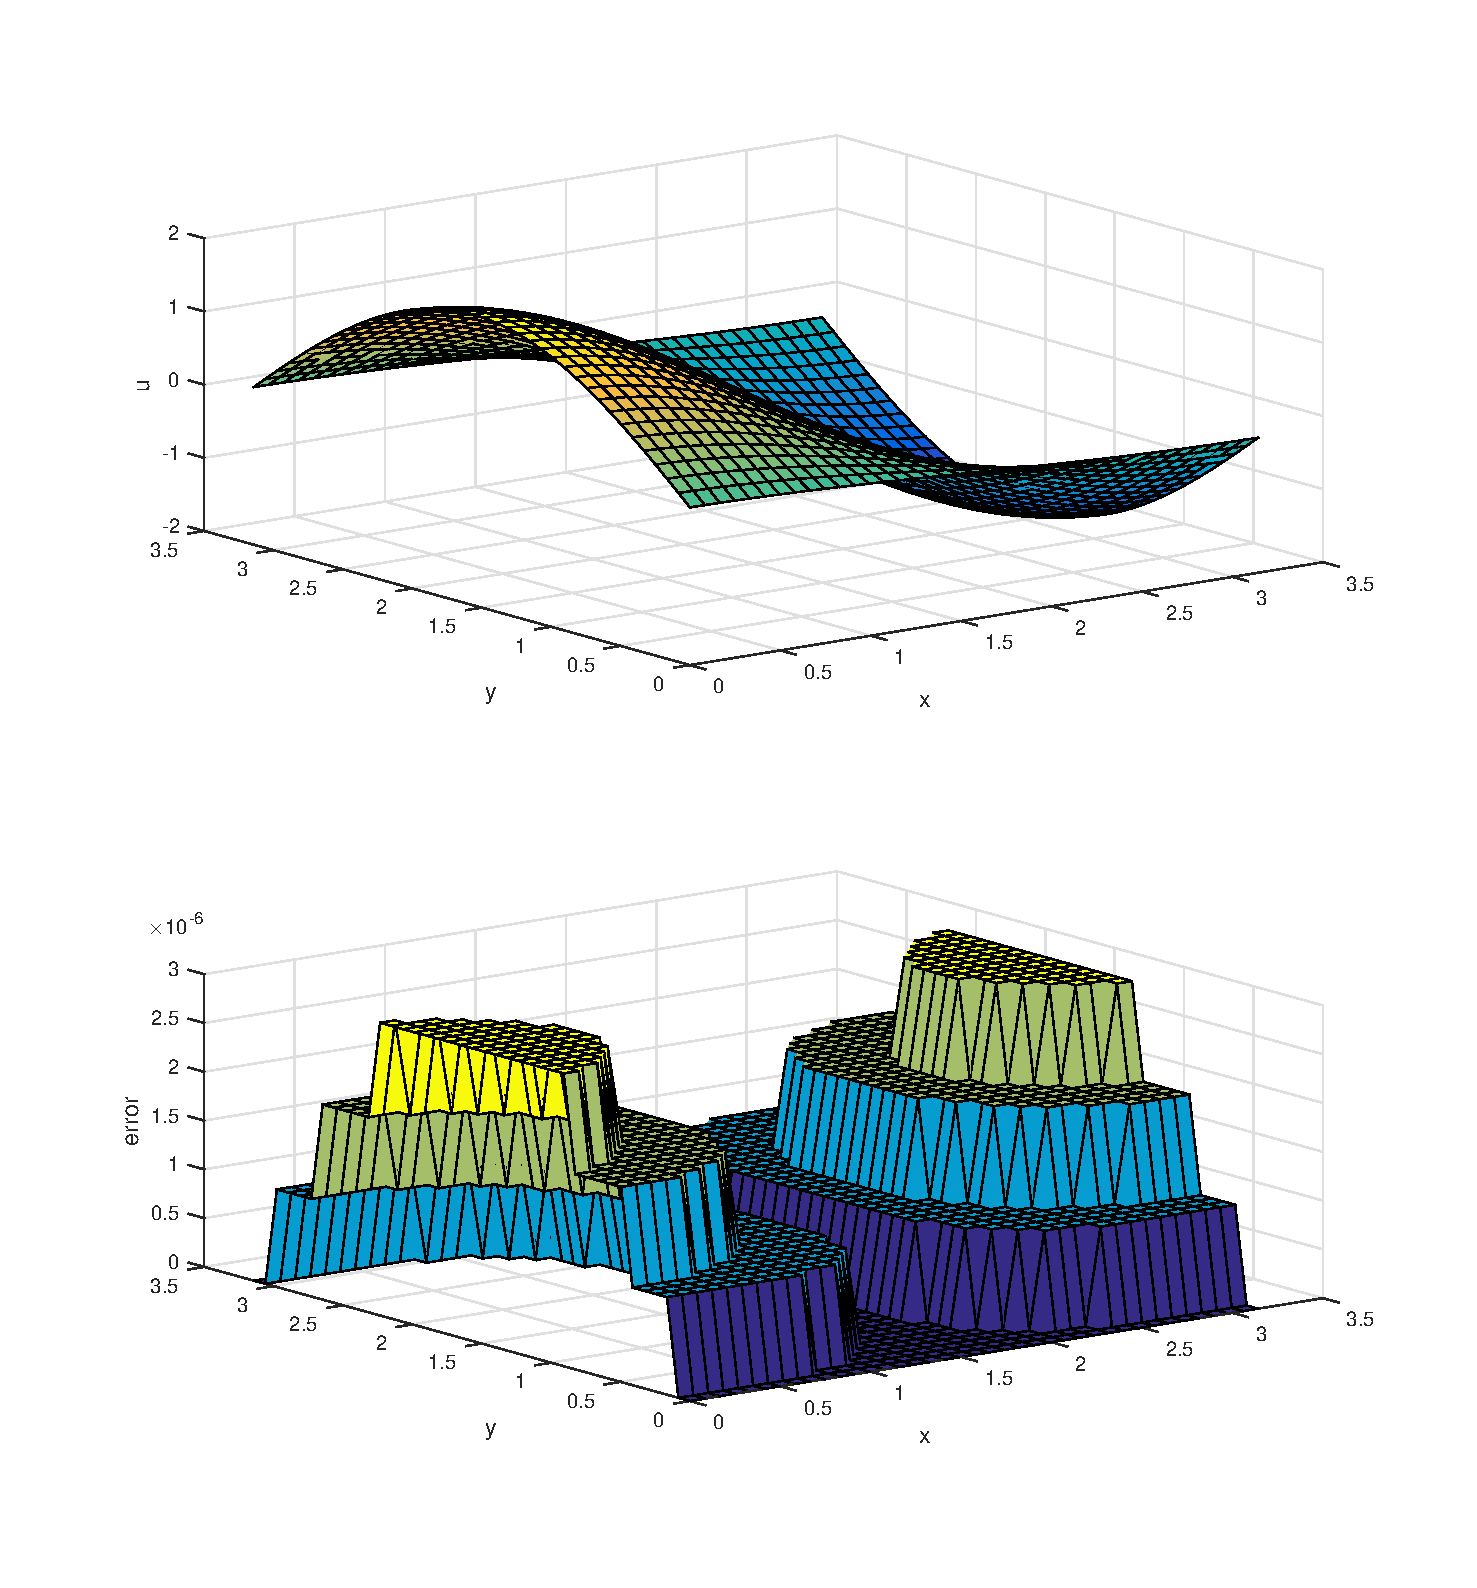
\includegraphics[width=3.5in]{csolnt01}
\caption{Solutions and Error at $t=0.1$}
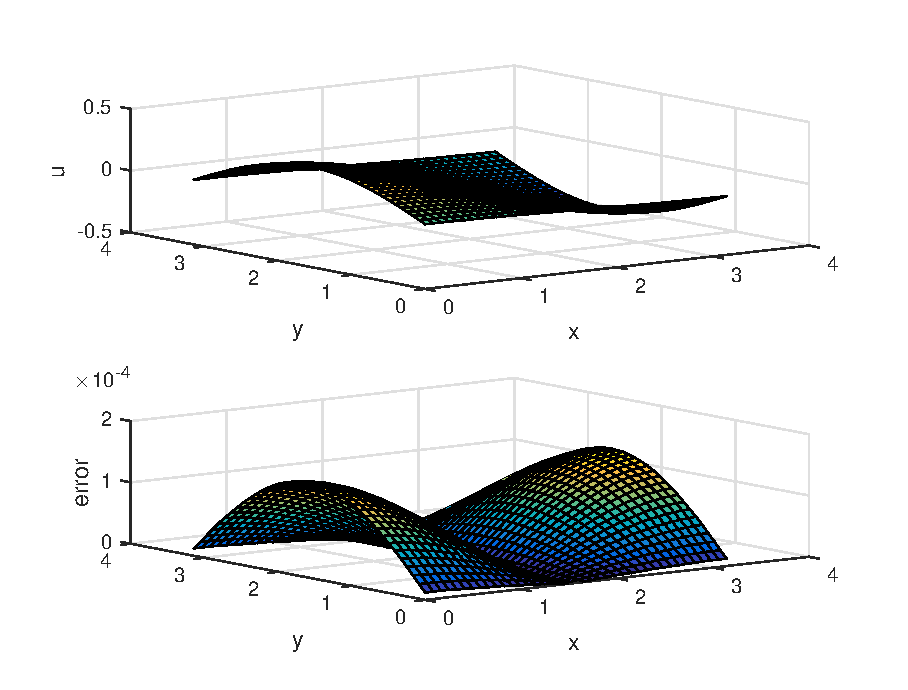
\includegraphics[width=3.5in]{csolnt1}\\
\caption{Solutions and Error at $t=1$}
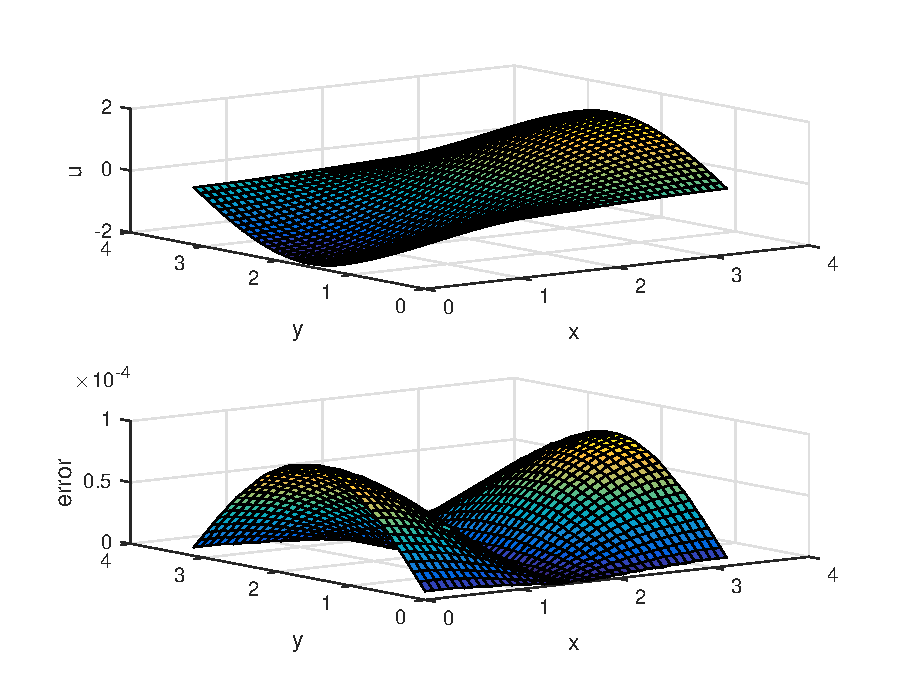
\includegraphics[width=3.5in]{csolnt2}
\caption{Solutions and Error at $t=2$}
\end{figure}
\eenum



\end{document}